\documentclass[12pt]{article}
\usepackage[T1]{fontenc}
%\usepackage[latin9]{inputenc}
\usepackage[utf8]{inputenc}
\usepackage[english]{babel}
\usepackage{amsmath}
\usepackage{amsfonts}
\usepackage{amssymb}
%\usepackage{setspace}
\usepackage{rotating}
\usepackage{graphics}
\usepackage{eurosym}
\usepackage[round]{natbib}
%\usepackage{graphicx}
%\usepackage{float} 				%allows you to float images
\usepackage{latexsym}
%\usepackage{bbding}
%\usepackage {moresize}
\usepackage{listings}
\usepackage{bbding}
\usepackage{blindtext}
\usepackage{hhline}
\usepackage{tikz}
\usetikzlibrary{trees}
%\usetikzlibrary{shapes,backgrounds}
%\usepackage{pgfplots}
%\usetikzlibrary{arrows}
\usepackage{enumitem}
%\doublespacing
%\usepackage{geometry}
\usepackage{amsthm}
\usepackage{color}
%\usepackage{array,multirow}
%\usepackage{subcaption}
%\usepackage{pst-plot}
%	\psset{xunit=15mm}
%\geometry{verbose,tmargin=1in,bmargin=1in,lmargin=.5in,rmargin=.5in}
\setlength{\parskip}{\bigskipamount}
\setlength{\parindent}{0pt}
\usepackage{multicol}

\newenvironment{problem}[3][Problem]{\begin{trivlist}
\item[\hskip \labelsep {\bfseries #1}\hskip \labelsep {\bfseries #2.}]}{\end{trivlist}}

\newcommand{\barr}{\bar{r}}
\newcommand{\ddx}{\frac{d}{dx}}
\newcommand{\infsum}{\sum_{n=1}^{\infty }}

\title{Problem Set 3 \thanks{Problems:4.5,4.8,4.9,4.11,4.12,4.14,4.16,4.22,4.34}}
\author{Ian McGroarty \\
	Course Number: 555.444}
\date{September 16, 2019}

\begin{document}

\maketitle
\newpage
%%%%%%%%%%%%%%%%%%%%%%%%%%%%%%%%%%%%%%%%%%%%%%%%%%%%%%%%
%%%%%%%%%%%%%%%%%%%%%%%%%%%%%%%%%%%%%%%%%%%%%%%%%%%%%%%%
%%%%%%%%%%%%%%%%%%%%%%%%%%%%%%%%%%%%%%%%%%%%%%%%%%%%%%%%
\begin{problem}{4.5}. Suppose that zero interst rates with continuous compounding are as follows: Calculate the forward interest rates for the 2nd 3rd, 4th, 5th, and 6th quarters. 

I use excel to perform these calculations. The forward rate formula s 
\begin{align*}
R_f &= \frac{R_2T_2 - R_1T_1}{T_2-T_1} && \text{Eqn 4.5, pg 90} 
\end{align*}
The resultant table is below: \\
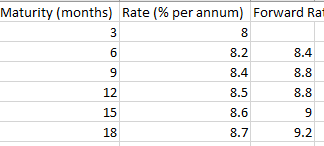
\includegraphics[width=0.75\textwidth ]{mod3_p1.png}
  \end{problem}

%%%%%%%%%%%%% NOT DONE %%%%%%%%%%%%%%%%%%%%%%%%%%%%%%%%%%%%%%%%%%% 
\begin{problem}{4.8}. What does duration tell you about the sensitivity of a bond portfolio to interest rates? What are the limitations of the duration measure?

Sorry this is going to be a long winded response as I try to explain duration to myself. Okay, so lets walk through this. First what is duration. In a nutshell, duration is how long it takes for you to get your money back. So lets think about that for a second. What is going to impact how long it takes for the investor to be repaid?
\begin{itemize}
\item Well the obvious choice is the maturity: The longer the maturity (ceteris paribus) the longer it will take for you to get your money back. So longer maturity = higher duration. 
\item Next obvious is the coupon payment: The higher the coupon payment the higher your inflow stream is and thus you get your money back faster. So higher coupon = lower duration.
\end{itemize}
Before we get into the third point which will finally answer this question (yield), lets take a closer look at what is going on with maturity and coupon. To do this we look at our next understanding of duration: the weighted average of of the time periods returns. This follows from the first part fairly well. The longer the maturity the higher the weights, the higher the coupon (ceteris paribus) the lower the weights need to be. This is particularly useful because now we an start to see how it links to yields. Since we are effectively discounting the time periods we can think of the duration as a way to measure the elasticity of bond price with respect to yield. Unforunately, similarly to elasticity, this assumes a linear relationship between price and yield (which would be a limitation of the duration calculation. 
\end{problem}

\begin{problem}{4.9}. What rate of interest with continuous compounding is equivalence to 15\% per annum with monthly compounding?

For this problem we can use equation 4.4 with $m=12$ times per year, and $R_m= 0.15$.
\begin{align*}
R_m &= m(e^{R_c/m} - 1) && \text{Eqn. 4.4, pg 83} \\ 
&= 12 \cdot (e^{.15/12-1}) \\ 
R_m &= 15.09\%
\end{align*}
\end{problem}


\begin{problem}{4.11}. Suppose that 6, 12, 18, 24, and 30 month zero rates are 4, 4.2, 4.4, 4.6, and 4.8 per annum with continuous compounding. Estimate the cash price of a bond with a face value of 100 that will mature in 30 months and pays a coupon of 4\% per annum semiannually. 

The coupon payment is \$4 made semiannually is \$2 and \$102 at 30 months. 
\begin{align*}
2e^{-0.04 \cdot 0.5} +& 2e^{-0.042 \cdot 1} + 2e^{-0.044 \cdot 1.5}+2e^{-0.046 \cdot 2} + 102e^{-0.048 \cdot 2.5} = 98.04
\end{align*}
\end{problem}

\begin{problem}{4.12}. A three year bond provides a coupon of 8\% semiannually and has a cash price of 104. What is the bond yield. 

The coupon payment is \$8 made semiannually is \$4 and \$104 at three years. Using the same method as above (q 4.11), but (with excel) trying various values of R. The bond yeild of a 3 year bond which provides a coupon of 8\% per annum is 6.4\%. 
\end{problem}


\begin{problem}{4.14}. Suppose that zero interst rates with continuous compounding are as follows: Calculate forward interest rates. 

Using the same method as problem 4.5: \\
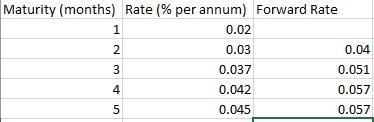
\includegraphics[width=0.75\textwidth]{mod3_p414.png}
\end{problem}

\begin{problem}{4.16}. A 10 year, 8\% coupon bond currently sells for \$90. A 10 year, 4\% coupon bond currently sells for \$80. What is the 10 year zero rate? 

The problem says to take out 2 long on the 4\% and one short on the  8\% so. The cash flow today is: $1*90 - 2*80 = -70$. So we pay a net \$70 for the position today. Now lets assume that the par value on each of these bonds is \$100 (because when is it ever not). So in 10 years we will receive \$200 from the long positions and pay \$100 from the short position to net \$100. We can say that this equals all the interest and principal which is received at year 10, (though Im not sure how the coupon prices play in here). Hence, we are simply able to use equation 4.3 (page 82):
\begin{align*}
100 &= 70\cdot e^{10R} && \text{Eqn. 4.3 pg 82} \\
ln(10/7) &= 10R \\
R &= 0.0357 
\end{align*}
\end{problem}

\begin{problem}{4.22}. A five year bond with a yield of 11\% (continuously compounded) pays an 8\% coupon at the end of each year. Formulas are below, calculations made in excel (also below) \\
\begin{align*}
\textbf{A. Bond Price} &= 8e^{-1\cdot0.11} + 8e^{-2\cdot0.11} + 8e^{-3\cdot0.11} + 8e^{-4\cdot0.11} + 108e^{-5\cdot0.11} = 86.801\\
\textbf{B. Duration} &= D = \frac{\Sigma t_ic_ie^{-yt_i}}{B}  = 4.256 \\
\textbf{C. Change in Yield} &= \Delta B = -B \cdot D \cdot \Delta y = -86.801 \cdot 4.256 \cdot -0.002 = 0.7388 \\
\end{align*}
\textbf{D. Verfiy} We see in the table below that the price at 10.8\% yield is $$87.543 \approx 86.801 + 0.7388$$
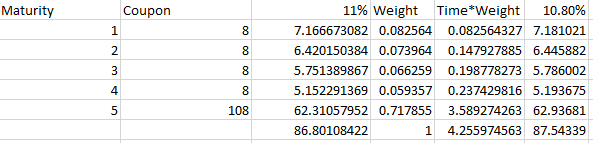
\includegraphics[width=0.75\textwidth]{mod3_p422.png}
\end{problem}

\begin{problem}{4.34}. The following table gives the price of bonds: 

\textbf{A. Calculate zero Rates}: We for 0.5 and 1.0 we need only solve $100=BondPrice \cdot e^{t\cdot R}$ for R. (Calculations shown in table below). For 1.5 year we have an annual coupon of 6.2 which is a semiannual coupon of 3.1. Using the zero rates for 0.5 and 1.0: 
\begin{align*}
100 &=  3.1e^{-0.040405*0.5} + 3.1e^{-0.0512} + 103.1e^{R\cdot 1.5}\\
& =  3.038001 + 2.945275 + 103.1e^{R\cdot 1.5} \\
0.0544 &= R \\
100 &=  4e^{-0.040405*0.5} + 4e^{-0.0512} + 4e^{.0544 \cdot 1.5} + 104e^{R\cdot 2} \\
0.0581 &= R
\end{align*}

\textbf{C. Par Yeild} Using $c=\frac{(100-100d)m}{A}$ on page 85, we can calculate the par yield. Ive included these calculations in the excel table below.

\textbf{D. Bond Price}  Estimate the bond price and yield of a two year bond providing a semiannual coupon of 7\% per annum. 
\begin{align*}
 3.5e^{-0.040405*0.5} + 3.5e^{-0.0512} + 3.5e^{.0544 \cdot 1.5} + 103.5e^{0.0581\cdot 2} &= 102.13 \\
 3.5e^{-y*0.5} + 3.5e^{-y} + 3.5e^{y \cdot 1.5} + 103.5e^{y\cdot 2} &= 102.13 \\
y&= 0.058. 
\end{align*}
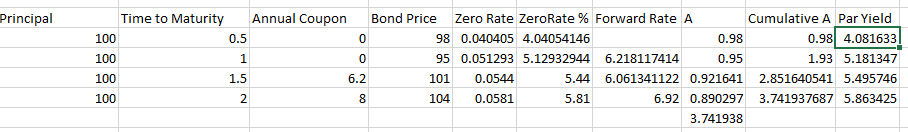
\includegraphics[width=\textwidth]{mod3_p434.png}


\end{problem}

\end{document}




% Set the overall layout of the tree




\tikzstyle{level 1}=[level distance=3.5cm, sibling distance=3.5cm]
\tikzstyle{level 2}=[level distance=3.5cm, sibling distance=2cm]

% Define styles for bags and leafs
\tikzstyle{bag} = [text width=4em, text centered]
\tikzstyle{end} = [circle, minimum width=3pt,fill, inner sep=0pt]

\begin{tikzpicture}[grow=right, sloped]
\node[bag] {Bag 1 $4W, 3B$}
    child {
        node[bag] {Bag 2 $4W, 5B$}        
            child {
                node[end, label=right:
                    {$P(W_1\cap W_2)=\frac{4}{7}\cdot\frac{4}{9}$}] {}
                edge from parent
                node[above] {$W$}
                node[below]  {$\frac{4}{9}$}
            }
            child {
                node[end, label=right:
                    {$P(W_1\cap B_2)=\frac{4}{7}\cdot\frac{5}{9}$}] {}
                edge from parent
                node[above] {$B$}
                node[below]  {$\frac{5}{9}$}
            }
            edge from parent 
            node[above] {$W$}
            node[below]  {$\frac{4}{7}$}
    }
    child {
        node[bag] {Bag 2 $3W, 6B$}        
        child {
                node[end, label=right:
                    {$P(B_1\cap W_2)=\frac{3}{7}\cdot\frac{3}{9}$}] {}
                edge from parent
                node[above] {$B$}
                node[below]  {$\frac{3}{9}$}
            }
            child {
                node[end, label=right:
                    {$P(B_1\cap B_2)=\frac{3}{7}\cdot\frac{6}{9}$}] {}
                edge from parent
                node[above] {$W$}
                node[below]  {$\frac{6}{9}$}
            }
        edge from parent         
            node[above] {$B$}
            node[below]  {$\frac{3}{7}$}
    };
\end{tikzpicture}


\section{Definitions}
\underline{Def: Forward Rate Formulas} (pg 79). The implied forward rate between times $t_1$ and $t_2$ is the rate of interset between those times that is consistent with a given spot rate curve. For Yearly compounding, the forward rate is:  
\begin{align*}
f_{i,j} =& [\frac{(1+s_j)^j}{(1+s_i)^i}]^{1/(j-i)}-1 \\
 e^{s(t_2)t_2} =& e^{s(t_1)t_1}e^{f_{t_1,t_2}(t_2-t_1)}
\end{align*}

\underline{Discount Factor Relation} The discount facot between periods i and j is defined as $$ d_{i,j}=[\frac{1}{1+f_{i,j}}]^{j-i}$$ These factors satisfy the compounding rule: $d_{i,k}=d_{i,j}d_{j,k}$\\

\underline{Def. Derivative (Ross pg 223)} Let F be a real valued function defined on an open interval contained a point a. We say f is differentiable at a, or f has derivative at a if the limit $$ f'(a) = \lim_{x \to a} \frac{f(x)-f(a)}{x-a} $$




https://www.investopedia.com/university/advancedbond/bond-pricing.asp
https://quant.stackexchange.com/questions/22288/duration-of-perpetual-bond
http://people.stern.nyu.edu/gyang/foundations/sample-final-solutions.html
http://pages.stern.nyu.edu/~jcarpen0/courses/b403333/07convexh.pdf
https://web.stanford.edu/class/msande247s/2009/summer%2009%20week%205/Bond%20Formula%20Sheet.pdf


\underline{Def: Forward Rate Formulas} (pg 79). The implied forward rate between times $t_1$ and $t_2$ is the rate of interset between those times that is consistent with a given spot rate curve. For Yearly compounding, the forward rate is:  
\begin{align*}
f_{i,j} =& [\frac{(1+s_j)^j}{(1+s_i)^i}]^{1/(j-i)}-1 \\
 e^{s(t_2)t_2} =& e^{s(t_1)t_1}e^{f_{t_1,t_2}(t_2-t_1)}
\end{align*}

\underline{Discount Factor Relation} The discount facot between periods i and j is defined as $$ d_{i,j}=[\frac{1}{1+f_{i,j}}]^{j-i}$$ These factors satisfy the compounding rule: $d_{i,k}=d_{i,j}d_{j,k}$\\

\underline{Def. Derivative (Ross pg 223)} Let F be a real valued function defined on an open interval contained a point a. We say f is differentiable at a, or f has derivative at a if the limit $$ f'(a) = \lim_{x \to a} \frac{f(x)-f(a)}{x-a} $$



\begin{align*}
\text{Maximize  } & 4x_1 +5x_2 +3x_3 +4.3x_4 + x_5 + 1.5x_6 + 2.5x_7 + 0.3x_8 + x_9 + 2x_{10} \\
\text{Subject to } & 2x_1 + 3x_2 + 1.5x_3 + 2.2x_4 +0.5x_5 +15x_6 + 2.5x_7 +0.1x_8 + 0.6x_9 + x_{10} \leq 5 \\ 
& x_1 + x_2 + x_3 + x_4 \leq 1 \\
& x_5 + x_6 + x_7 \leq 1 \\
& x_8 + x_9 + x_{10} \leq 1 \\
\end{align*}